\documentclass[twoside]{book}

% Packages required by doxygen
\usepackage{calc}
\usepackage{doxygen}
\usepackage{graphicx}
\usepackage[utf8]{inputenc}
\usepackage{makeidx}
\usepackage{multicol}
\usepackage{multirow}
\usepackage{textcomp}
\usepackage[table]{xcolor}

% Font selection
\usepackage[T1]{fontenc}
\usepackage{mathptmx}
\usepackage[scaled=.90]{helvet}
\usepackage{courier}
\usepackage{amssymb}
\usepackage{sectsty}
\renewcommand{\familydefault}{\sfdefault}
\allsectionsfont{%
  \fontseries{bc}\selectfont%
  \color{darkgray}%
}
\renewcommand{\DoxyLabelFont}{%
  \fontseries{bc}\selectfont%
  \color{darkgray}%
}

% Page & text layout
\usepackage{geometry}
\geometry{%
  a4paper,%
  top=2.5cm,%
  bottom=2.5cm,%
  left=2.5cm,%
  right=2.5cm%
}
\tolerance=750
\hfuzz=15pt
\hbadness=750
\setlength{\emergencystretch}{15pt}
\setlength{\parindent}{0cm}
\setlength{\parskip}{0.2cm}
\makeatletter
\renewcommand{\paragraph}{%
  \@startsection{paragraph}{4}{0ex}{-1.0ex}{1.0ex}{%
    \normalfont\normalsize\bfseries\SS@parafont%
  }%
}
\renewcommand{\subparagraph}{%
  \@startsection{subparagraph}{5}{0ex}{-1.0ex}{1.0ex}{%
    \normalfont\normalsize\bfseries\SS@subparafont%
  }%
}
\makeatother

% Headers & footers
\usepackage{fancyhdr}
\pagestyle{fancyplain}
\fancyhead[LE]{\fancyplain{}{\bfseries\thepage}}
\fancyhead[CE]{\fancyplain{}{}}
\fancyhead[RE]{\fancyplain{}{\bfseries\leftmark}}
\fancyhead[LO]{\fancyplain{}{\bfseries\rightmark}}
\fancyhead[CO]{\fancyplain{}{}}
\fancyhead[RO]{\fancyplain{}{\bfseries\thepage}}
\fancyfoot[LE]{\fancyplain{}{}}
\fancyfoot[CE]{\fancyplain{}{}}
\fancyfoot[RE]{\fancyplain{}{\bfseries\scriptsize Generated on Mon Jun 9 2014 11\-:45\-:58 for My Project by Doxygen }}
\fancyfoot[LO]{\fancyplain{}{\bfseries\scriptsize Generated on Mon Jun 9 2014 11\-:45\-:58 for My Project by Doxygen }}
\fancyfoot[CO]{\fancyplain{}{}}
\fancyfoot[RO]{\fancyplain{}{}}
\renewcommand{\footrulewidth}{0.4pt}
\renewcommand{\chaptermark}[1]{%
  \markboth{#1}{}%
}
\renewcommand{\sectionmark}[1]{%
  \markright{\thesection\ #1}%
}

% Indices & bibliography
\usepackage{natbib}
\usepackage[titles]{tocloft}
\setcounter{tocdepth}{3}
\setcounter{secnumdepth}{5}
\makeindex

% Hyperlinks (required, but should be loaded last)
\usepackage{ifpdf}
\ifpdf
  \usepackage[pdftex,pagebackref=true]{hyperref}
\else
  \usepackage[ps2pdf,pagebackref=true]{hyperref}
\fi
\hypersetup{%
  colorlinks=true,%
  linkcolor=blue,%
  citecolor=blue,%
  unicode%
}

% Custom commands
\newcommand{\clearemptydoublepage}{%
  \newpage{\pagestyle{empty}\cleardoublepage}%
}


%===== C O N T E N T S =====

\begin{document}

% Titlepage & ToC
\hypersetup{pageanchor=false}
\pagenumbering{roman}
\begin{titlepage}
\vspace*{7cm}
\begin{center}%
{\Large My Project }\\
\vspace*{1cm}
{\large Generated by Doxygen 1.8.6}\\
\vspace*{0.5cm}
{\small Mon Jun 9 2014 11:45:58}\\
\end{center}
\end{titlepage}
\clearemptydoublepage
\tableofcontents
\clearemptydoublepage
\pagenumbering{arabic}
\hypersetup{pageanchor=true}

%--- Begin generated contents ---
\chapter{Hierarchical Index}
\section{Class Hierarchy}
This inheritance list is sorted roughly, but not completely, alphabetically\-:\begin{DoxyCompactList}
\item \contentsline{section}{Cards}{\pageref{class_cards}}{}
\item \contentsline{section}{Cash\-Out}{\pageref{class_cash_out}}{}
\item \contentsline{section}{Horse\-Race}{\pageref{class_horse_race}}{}
\begin{DoxyCompactList}
\item \contentsline{section}{Rivalh1}{\pageref{class_rivalh1}}{}
\item \contentsline{section}{Rivalh2}{\pageref{class_rivalh2}}{}
\item \contentsline{section}{Rivalh3}{\pageref{class_rivalh3}}{}
\item \contentsline{section}{User\-Horse}{\pageref{class_user_horse}}{}
\end{DoxyCompactList}
\item \contentsline{section}{Keno}{\pageref{struct_keno}}{}
\end{DoxyCompactList}

\chapter{Class Index}
\section{Class List}
Here are the classes, structs, unions and interfaces with brief descriptions\-:\begin{DoxyCompactList}
\item\contentsline{section}{\hyperlink{struct_player}{Player} }{\pageref{struct_player}}{}
\item\contentsline{section}{\hyperlink{structuser}{user} }{\pageref{structuser}}{}
\end{DoxyCompactList}

\chapter{Class Documentation}
\hypertarget{class_cards}{\section{Cards Class Reference}
\label{class_cards}\index{Cards@{Cards}}
}
\subsection*{Public Member Functions}
\begin{DoxyCompactItemize}
\item 
\hypertarget{class_cards_a6edf386b9d83a2c693e4a5b9f0bebf0c}{{\bfseries Cards} (int)}\label{class_cards_a6edf386b9d83a2c693e4a5b9f0bebf0c}

\item 
\hypertarget{class_cards_a5172d2158510ffb70c5b17eafa1d8df7}{void {\bfseries fill\-Deck} (int x)}\label{class_cards_a5172d2158510ffb70c5b17eafa1d8df7}

\item 
\hypertarget{class_cards_a94335b21943e9f10b76b74bb7ac4a62a}{int {\bfseries prnt} (int)}\label{class_cards_a94335b21943e9f10b76b74bb7ac4a62a}

\end{DoxyCompactItemize}


The documentation for this class was generated from the following files\-:\begin{DoxyCompactItemize}
\item 
card\-\_\-check.\-h\item 
card\-\_\-check.\-cpp\end{DoxyCompactItemize}

\hypertarget{class_cash_out}{\section{Cash\-Out Class Reference}
\label{class_cash_out}\index{Cash\-Out@{Cash\-Out}}
}
\subsection*{Public Member Functions}
\begin{DoxyCompactItemize}
\item 
\hypertarget{class_cash_out_aeb3c320946b4335d589547c21a139a54}{{\bfseries Cash\-Out} (float)}\label{class_cash_out_aeb3c320946b4335d589547c21a139a54}

\end{DoxyCompactItemize}
\subsection*{Protected Attributes}
\begin{DoxyCompactItemize}
\item 
\hypertarget{class_cash_out_a00dda22cfcc6088c0a7b0303dcd79502}{float {\bfseries total}}\label{class_cash_out_a00dda22cfcc6088c0a7b0303dcd79502}

\end{DoxyCompactItemize}


The documentation for this class was generated from the following file\-:\begin{DoxyCompactItemize}
\item 
Cash\-\_\-out.\-h\end{DoxyCompactItemize}

\hypertarget{class_horse_race}{\section{Horse\-Race Class Reference}
\label{class_horse_race}\index{Horse\-Race@{Horse\-Race}}
}
Inheritance diagram for Horse\-Race\-:\begin{figure}[H]
\begin{center}
\leavevmode
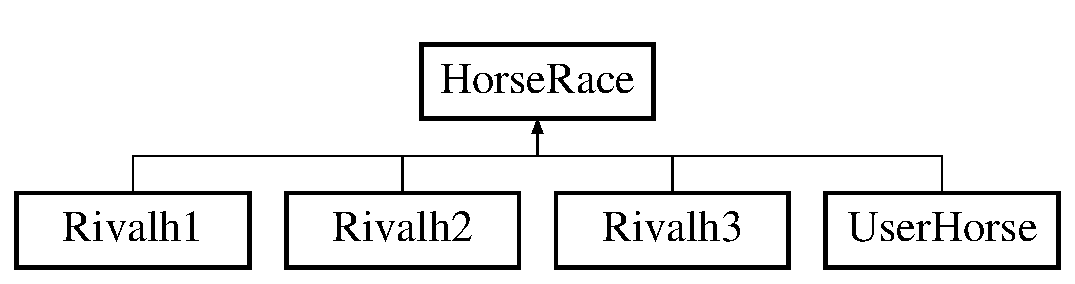
\includegraphics[height=2.000000cm]{class_horse_race}
\end{center}
\end{figure}
\subsection*{Public Member Functions}
\begin{DoxyCompactItemize}
\item 
\hypertarget{class_horse_race_aeb7d6f73ffdc7440e7eaf3d0761de6e5}{void {\bfseries set\-Distance} (int x)}\label{class_horse_race_aeb7d6f73ffdc7440e7eaf3d0761de6e5}

\end{DoxyCompactItemize}
\subsection*{Protected Attributes}
\begin{DoxyCompactItemize}
\item 
\hypertarget{class_horse_race_a21c58b9c94ac0763fc8b8f02bb07a638}{int {\bfseries advance}}\label{class_horse_race_a21c58b9c94ac0763fc8b8f02bb07a638}

\end{DoxyCompactItemize}


The documentation for this class was generated from the following file\-:\begin{DoxyCompactItemize}
\item 
main.\-cpp\end{DoxyCompactItemize}

\hypertarget{struct_keno}{\section{Keno Struct Reference}
\label{struct_keno}\index{Keno@{Keno}}
}
\subsection*{Public Attributes}
\begin{DoxyCompactItemize}
\item 
\hypertarget{struct_keno_a72026b482f694ca0523bf6823bfa5398}{int {\bfseries Random}}\label{struct_keno_a72026b482f694ca0523bf6823bfa5398}

\item 
\hypertarget{struct_keno_a4527cabf825f14d2492376f2d9b5d575}{int {\bfseries Self}}\label{struct_keno_a4527cabf825f14d2492376f2d9b5d575}

\item 
\hypertarget{struct_keno_a4d41b7c435352827b1a62d92d3f97d8b}{int {\bfseries st\-Draw}}\label{struct_keno_a4d41b7c435352827b1a62d92d3f97d8b}

\item 
\hypertarget{struct_keno_a6f68b76cd2ace9ed037749080ff56051}{int {\bfseries n\-Draw}}\label{struct_keno_a6f68b76cd2ace9ed037749080ff56051}

\item 
\hypertarget{struct_keno_a8a667845562f6ab7c92d56d59ce9cf10}{int {\bfseries counter}}\label{struct_keno_a8a667845562f6ab7c92d56d59ce9cf10}

\end{DoxyCompactItemize}


The documentation for this struct was generated from the following file\-:\begin{DoxyCompactItemize}
\item 
main.\-cpp\end{DoxyCompactItemize}

\hypertarget{class_rivalh1}{\section{Rivalh1 Class Reference}
\label{class_rivalh1}\index{Rivalh1@{Rivalh1}}
}
Inheritance diagram for Rivalh1\-:\begin{figure}[H]
\begin{center}
\leavevmode
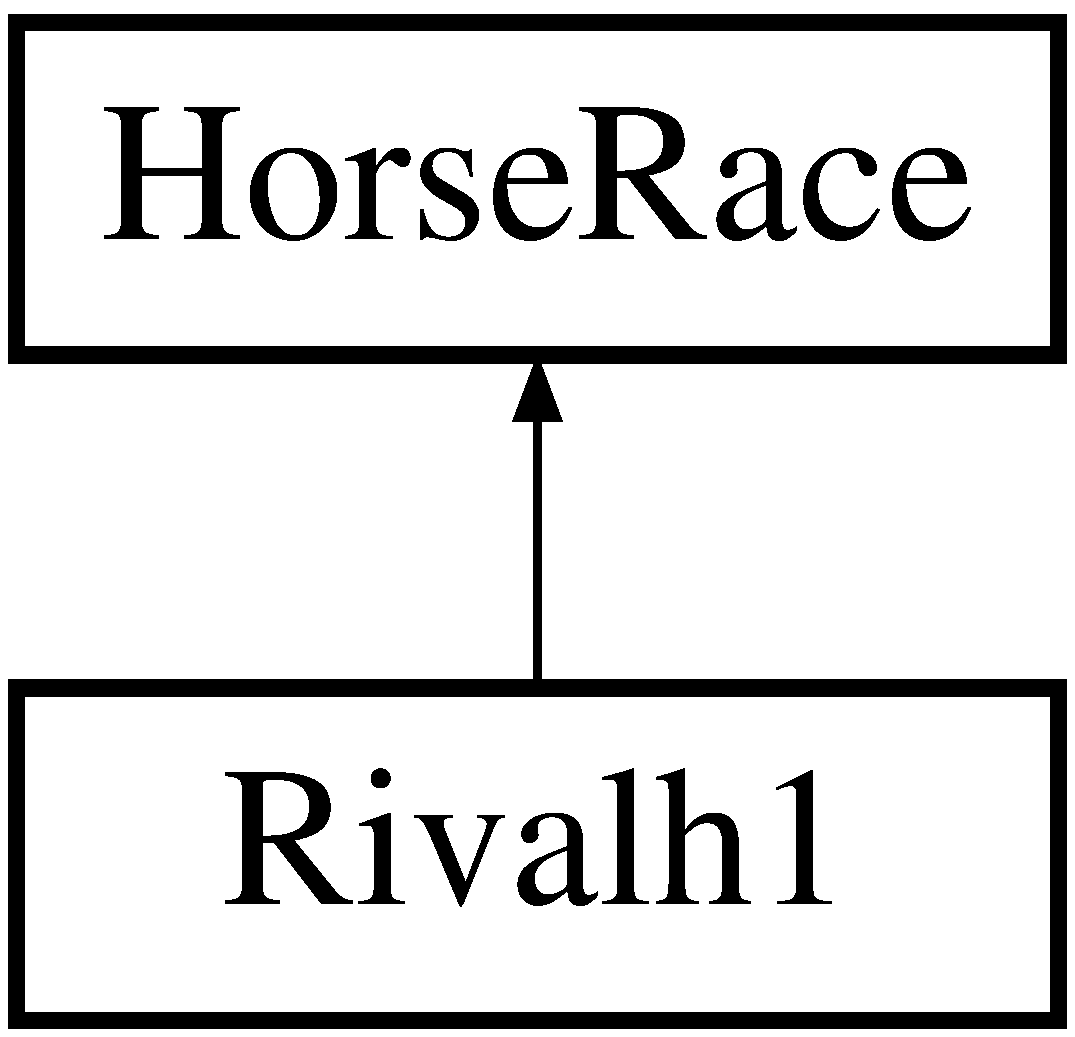
\includegraphics[height=2.000000cm]{class_rivalh1}
\end{center}
\end{figure}
\subsection*{Public Member Functions}
\begin{DoxyCompactItemize}
\item 
\hypertarget{class_rivalh1_a39ab092fc5a0fdd2ed04e742c0052e34}{void {\bfseries rand\-Horse1} ()}\label{class_rivalh1_a39ab092fc5a0fdd2ed04e742c0052e34}

\end{DoxyCompactItemize}
\subsection*{Additional Inherited Members}


The documentation for this class was generated from the following file\-:\begin{DoxyCompactItemize}
\item 
main.\-cpp\end{DoxyCompactItemize}

\hypertarget{class_rivalh2}{\section{Rivalh2 Class Reference}
\label{class_rivalh2}\index{Rivalh2@{Rivalh2}}
}
Inheritance diagram for Rivalh2\-:\begin{figure}[H]
\begin{center}
\leavevmode
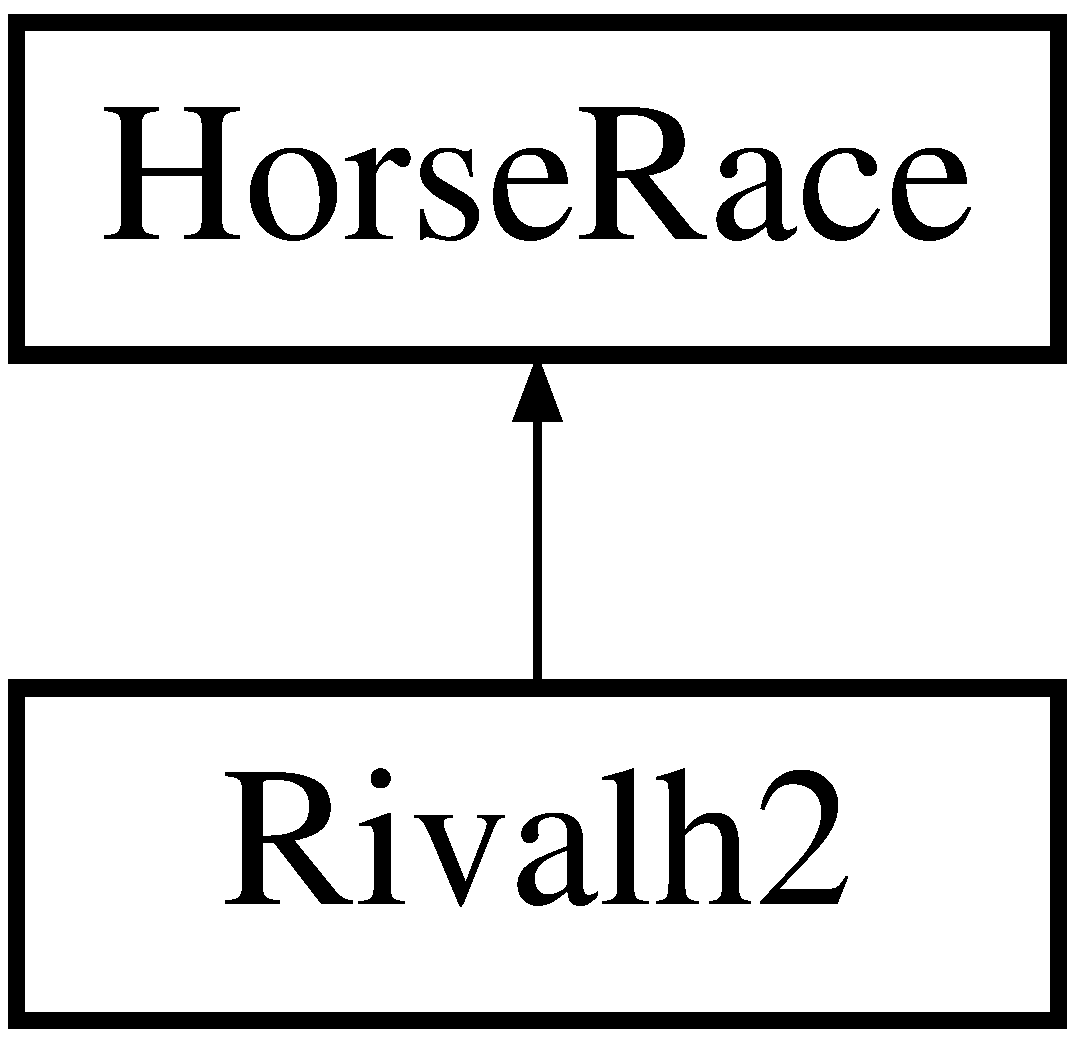
\includegraphics[height=2.000000cm]{class_rivalh2}
\end{center}
\end{figure}
\subsection*{Public Member Functions}
\begin{DoxyCompactItemize}
\item 
\hypertarget{class_rivalh2_aa72fd70dfdb1daa87b23451751d535ce}{void {\bfseries rand\-Horse2} ()}\label{class_rivalh2_aa72fd70dfdb1daa87b23451751d535ce}

\end{DoxyCompactItemize}
\subsection*{Additional Inherited Members}


The documentation for this class was generated from the following file\-:\begin{DoxyCompactItemize}
\item 
main.\-cpp\end{DoxyCompactItemize}

\hypertarget{class_rivalh3}{\section{Rivalh3 Class Reference}
\label{class_rivalh3}\index{Rivalh3@{Rivalh3}}
}
Inheritance diagram for Rivalh3\-:\begin{figure}[H]
\begin{center}
\leavevmode
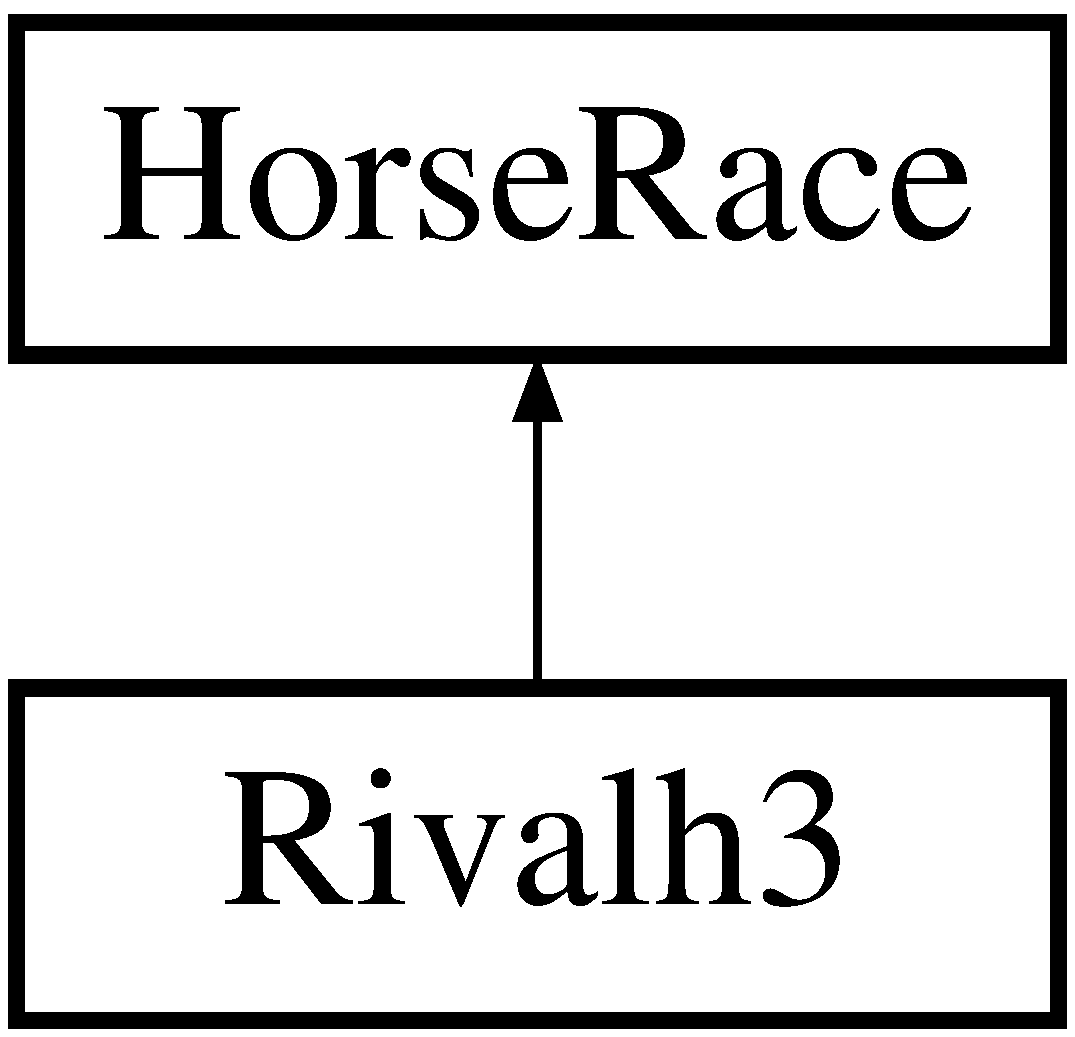
\includegraphics[height=2.000000cm]{class_rivalh3}
\end{center}
\end{figure}
\subsection*{Public Member Functions}
\begin{DoxyCompactItemize}
\item 
\hypertarget{class_rivalh3_a2a325fe04be1bd0a15a9c05353934e52}{void {\bfseries rand\-Horse3} ()}\label{class_rivalh3_a2a325fe04be1bd0a15a9c05353934e52}

\end{DoxyCompactItemize}
\subsection*{Additional Inherited Members}


The documentation for this class was generated from the following file\-:\begin{DoxyCompactItemize}
\item 
main.\-cpp\end{DoxyCompactItemize}

\hypertarget{class_user_horse}{\section{User\-Horse Class Reference}
\label{class_user_horse}\index{User\-Horse@{User\-Horse}}
}
Inheritance diagram for User\-Horse\-:\begin{figure}[H]
\begin{center}
\leavevmode
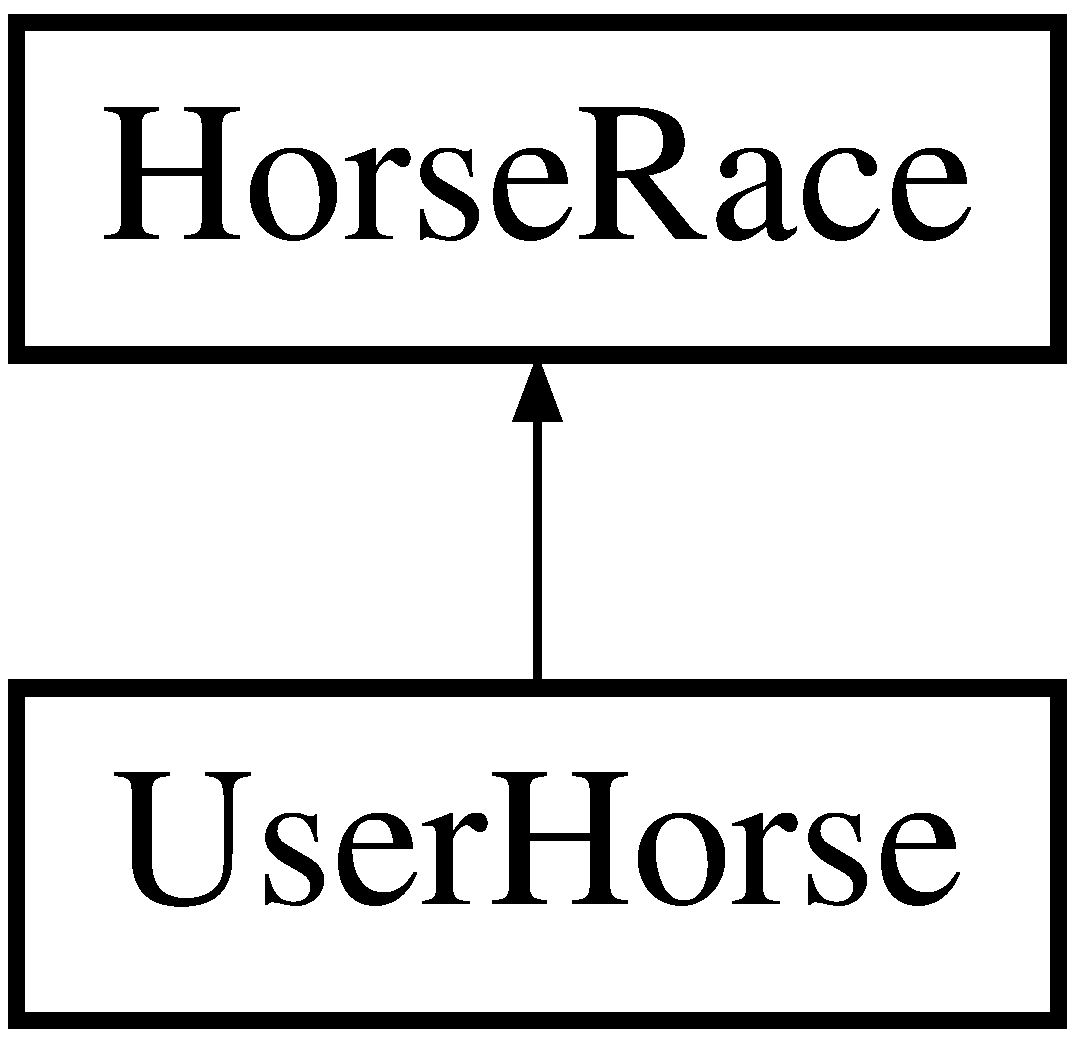
\includegraphics[height=2.000000cm]{class_user_horse}
\end{center}
\end{figure}
\subsection*{Public Member Functions}
\begin{DoxyCompactItemize}
\item 
\hypertarget{class_user_horse_a2e6c6cd477af7664de33a466b009b0d4}{void {\bfseries My\-Horse} ()}\label{class_user_horse_a2e6c6cd477af7664de33a466b009b0d4}

\end{DoxyCompactItemize}
\subsection*{Additional Inherited Members}


The documentation for this class was generated from the following file\-:\begin{DoxyCompactItemize}
\item 
main.\-cpp\end{DoxyCompactItemize}

%--- End generated contents ---

% Index
\newpage
\phantomsection
\addcontentsline{toc}{chapter}{Index}
\printindex

\end{document}
